\lfoot{Autor: Fitim Faiku}
\subsection{Fahrkomfortanalyse}


Autofahrten werden durch die Bequemlichkeit der Fahrt bewertet. 
Diese Bewertung fällt meistens aus den Faktoren wie stark ein Fahrer beschleunigt und in welcher Geschwindigkeit er um eine Kurve fährt. Je nach dem erhöhen sich die Beschleunigungskräfte und die Fahrt wird mit immer größeren Beschelunigungskräften unangenehmer.
Um einen KFZ-Einsteiger mit möglichst Informativen Daten zu \"bewerten\" haben wir uns einen Kammshen Kreis als Hilfe genommen.

\subsubsection{Kammsher Kreis }
Ein Kammsher Kreis ist ein ein Kreis in dem durch Polarkoordinaten die Extremwerte einer Fahrt eingezeichnet sind.
Der Kreis ist so aufgebaut, dass in Norden de Bremskräfte angezeigt werden, in Süden alle Beschleunigungen, im Westen die Rechtskurven und Osten die Linkskurven.
Es ist also alles verkehrt.
\begin{figure}[!htb]\centering
	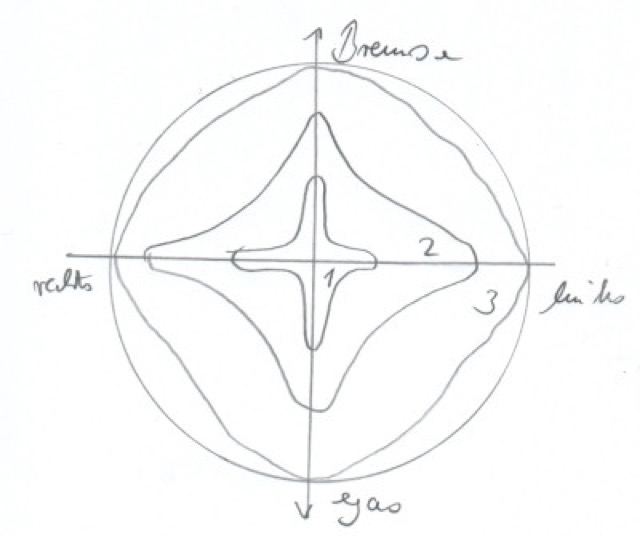
\includegraphics[width=0.5\textwidth]{images/kammsherkreis}
	\caption{Kammsherkreis \cite{FAIF.CH3-fahrkomfortanalyse.KammscherKreis}}\label{Fig:Kammsher-Kreis}
\end{figure}

\subsubsection{Implementierung}
Um diesen Kammschen Kreis richtig darzustellen haben wir uns die Klasse canvas als Hilfe genommen, wobei sie von Graphics erbt und wir somit auf einer Fläche zeichnen können.
Um die Punkte des Kammshen Kreises zu zeichnen habe ich mir alle phi Winkel, welche zufällig generiert werden auf oder abgerundet. Das wird gemacht, um 72 Punkte in 5er Schritten zu Zeichnen.  


\lstinputlisting[caption=Runden-Methode, style=javastyle]{code/Runden.java}

\lstinputlisting[caption=Draw, style=javastyle]{code/ChartView.java}
Um den Kammshen-Kreis zu zeichnen habe ich die OnDraw Methode ueberschrieben, weiters speichere ich alle generierten Werte in einer Liste welche in einer For-Schleife gezeichnet werden.